\chapter{Week 3: Sept. 15 - Oct. 1}
\label{week:3}
\section{Tensorflow Example Continued}
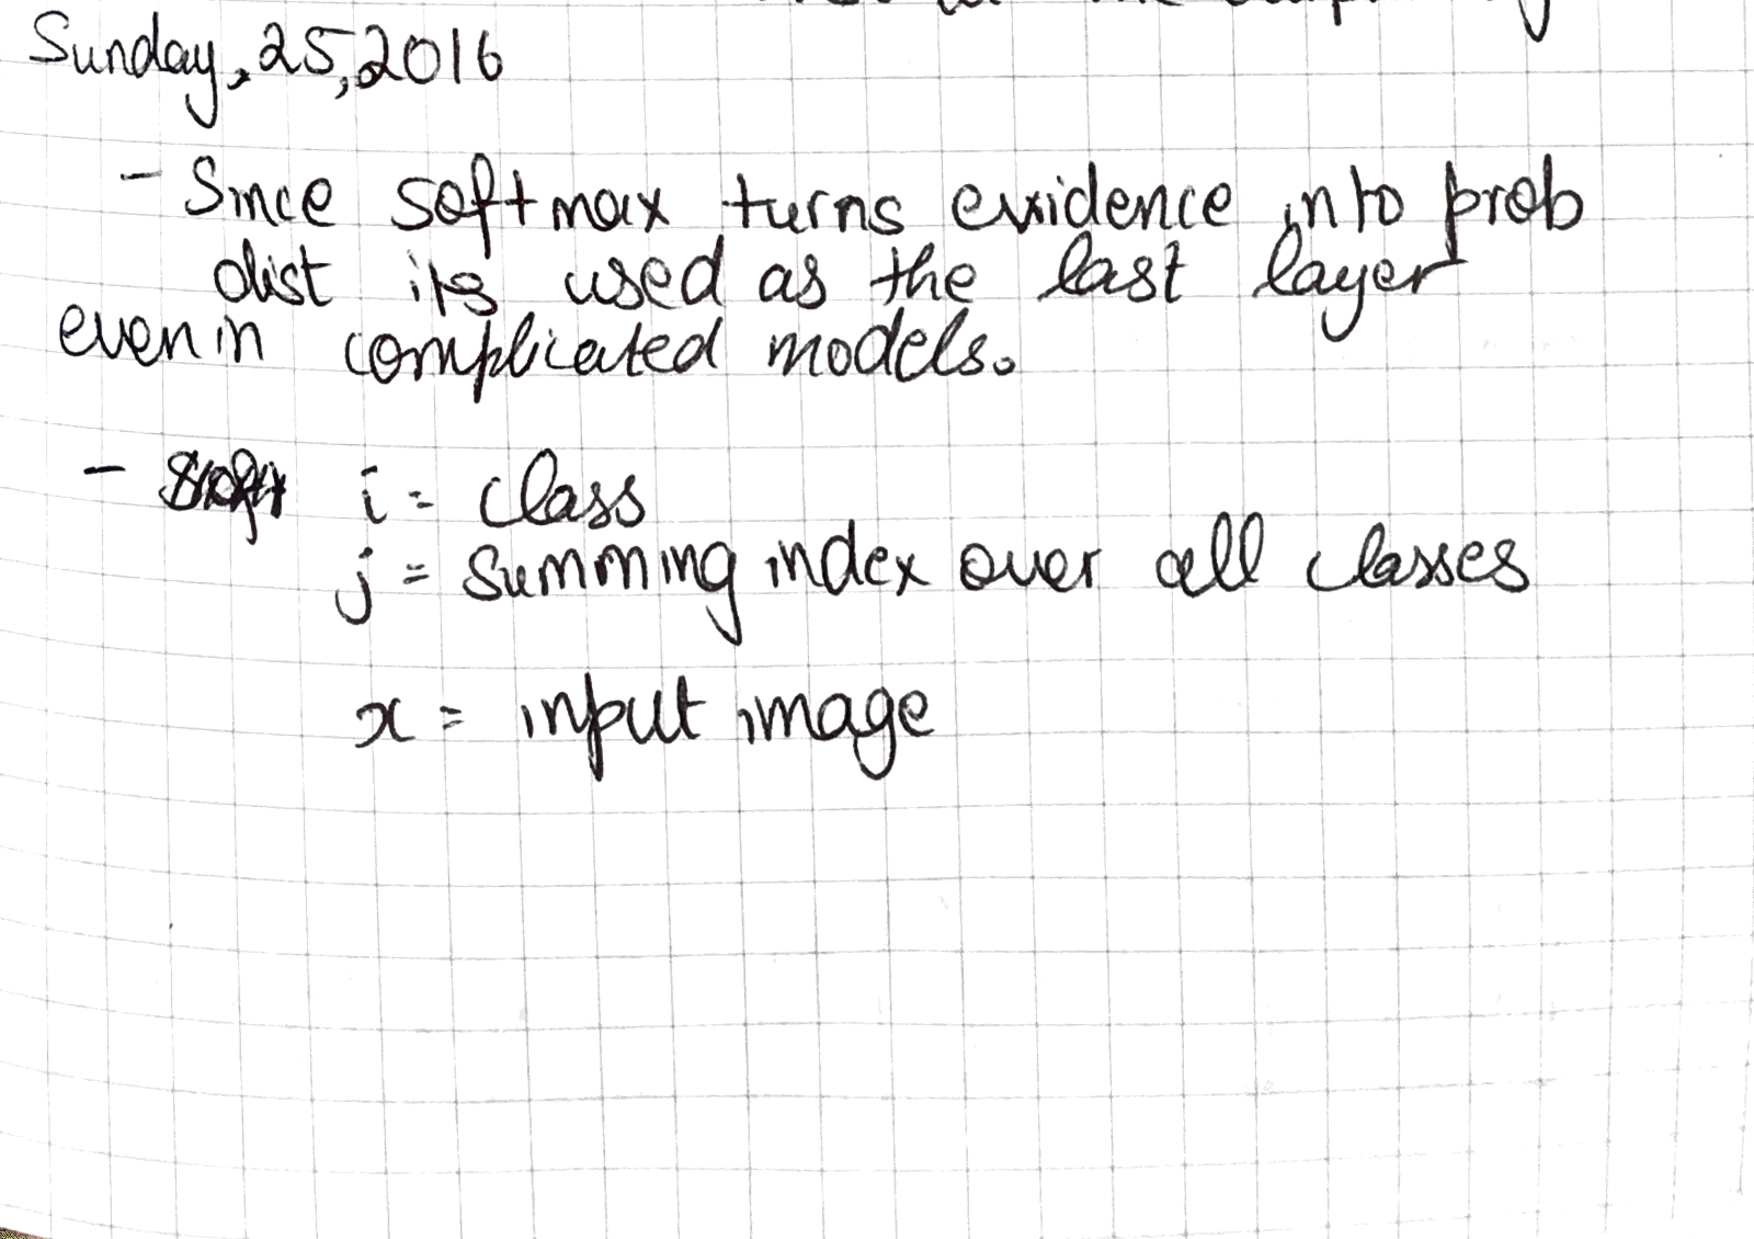
\includepdf[scale=1.0,pages=1]{../pdfs/Sept25-MNIST.pdf}
\includepdf[scale=1.0,pages=2-4]{../pdfs/Sept25-MNIST.pdf}
\section{Back Propagation}
\begin{itemize}
	\item Reverse mode differentiation
	\item Regular chain rule gives you the derviative of the output with respect to one input/node
	\item Doing that for all nodes is intractable
	\item To extend this to find $\frac{\partial output}{\partial}$ with respect to all nodes and inputs in the neural net/graph you start using the chain rule from the other end (output) and go till the input layer. This is essential for neural networks. \cite{backprop}
\end{itemize}